% THIS IS AN EXAMPLE DOCUMENT FOR VLDB 2012
% based on ACM SIGPROC-SP.TEX VERSION 2.7
% Modified by  Gerald Weber <gerald@cs.auckland.ac.nz>
% Removed the requirement to include *bbl file in here. (AhmetSacan, Sep2012)
% Fixed the equation on page 3 to prevent line overflow. (AhmetSacan, Sep2012)

\documentclass{vldb}
\usepackage{graphicx}
\usepackage{balance}  % for  \balance command ON LAST PAGE  (only there!)
\usepackage[utf8x]{inputenc}
\usepackage[colorinlistoftodos]{todonotes}
\usepackage{adjustbox}

% Include information below and uncomment for camera ready
\vldbTitle{Twitter data serialization methods and benchmarks}
\vldbAuthors{Ben Trovato, G. K. M. Tobin, Lars Th{\sf{\o}}rv{$\ddot{\mbox{a}}$}ld, Lawrence P. Leipuner, Sean Fogarty, Charles Palmer, John Smith, Julius P.~Kumquat, and Ahmet Sacan}
\vldbDOI{https://doi.org/10.14778/xxxxxxx.xxxxxxx}
\vldbVolume{12}
\vldbNumber{xxx}
\vldbYear{2019}

\begin{document}

% ****************** TITLE ****************************************

\title{Twitter data serialization methods and benchmarks}


% possible, but not really needed or used for PVLDB:
%\subtitle{[Extended Abstract]
%\titlenote{A full version of this paper is available as\textit{Author's Guide to Preparing ACM SIG Proceedings Using \LaTeX$2_\epsilon$\ and BibTeX} at \texttt{www.acm.org/eaddress.htm}}}

% ****************** AUTHORS **************************************

% You need the command \numberofauthors to handle the 'placement
% and alignment' of the authors beneath the title.
%
% For aesthetic reasons, we recommend 'three authors at a time'
% i.e. three 'name/affiliation blocks' be placed beneath the title.
%
% NOTE: You are NOT restricted in how many 'rows' of
% "name/affiliations" may appear. We just ask that you restrict
% the number of 'columns' to three.
%
% Because of the available 'opening page real-estate'
% we ask you to refrain from putting more than six authors
% (two rows with three columns) beneath the article title.
% More than six makes the first-page appear very cluttered indeed.
%
% Use the \alignauthor commands to handle the names
% and affiliations for an 'aesthetic maximum' of six authors.
% Add names, affiliations, addresses for
% the seventh etc. author(s) as the argument for the
% \additionalauthors command.
% These 'additional authors' will be output/set for you
% without further effort on your part as the last section in
% the body of your article BEFORE References or any Appendices.

\numberofauthors{3} %  in this sample file, there are a *total*
% of EIGHT authors. SIX appear on the 'first-page' (for formatting
% reasons) and the remaining two appear in the \additionalauthors section.

\author{
% You can go ahead and credit any number of authors here,
% e.g. one 'row of three' or two rows (consisting of one row of three
% and a second row of one, two or three).
%
% The command \alignauthor (no curly braces needed) should
% precede each author name, affiliation/snail-mail address and
% e-mail address. Additionally, tag each line of
% affiliation/address with \affaddr, and tag the
% e-mail address with \email.
%
% 1st. author
\alignauthor
	  Kia Teymourian \\
       \affaddr{Boston University}\\
       %\affaddr{1932 Wallamaloo Lane}\\
       %\affaddr{Wallamaloo, New Zealand}\\
       \email{kiat@bu.edu}
% 2nd. author
\alignauthor
	   Saeed Fathollahzadeh \\
       \affaddr{Free University of Bozen-Bolzano}\\
       %\affaddr{P.O. Box 1212}\\
       %\affaddr{Dublin, Ohio 43017-6221}\\
       \email{s.fathollahzadeh@gmail.com}
% 3rd. author
\alignauthor 
	  Chris Jermaine \\
       \affaddr{Rice University}\\
       %\affaddr{1 Th{\large{\sf{\o}}}rv{$\ddot{\mbox{a}}$}ld Circle}\\
       %\affaddr{Hekla, Iceland}\\
       \email{cmj4@rice.edu}

}
% There's nothing stopping you putting the seventh, eighth, etc.
% author on the opening page (as the 'third row') but we ask,
% for aesthetic reasons that you place these 'additional authors'
% in the \additional authors block, viz.
\additionalauthors{Additional authors: John Smith (The Th{\o}rv\"{a}ld Group, {\texttt{jsmith@affiliation.org}}), Julius P.~Kumquat
(The \raggedright{Kumquat} Consortium, {\small \texttt{jpkumquat@consortium.net}}), and Ahmet Sacan (Drexel University, {\small \texttt{ahmetdevel@gmail.com}})}
\date{30 July 1999}
% Just remember to make sure that the TOTAL number of authors
% is the number that will appear on the first page PLUS the
% number that will appear in the \additionalauthors section.


\maketitle


\begin{abstract}
\todo[inline]{abstract}
\end{abstract}
\section{Introduction}
\todo[inline]{Introduction}
The contribution of our work are the following:
\begin{enumerate}
	\item we implement all serialization methods in C++ and Java programming language in a single thread system. But, we evaluate the methods with $task set$ for restrict run the method on a special core and without $task set$ to allow run method on the arbitrary cores. In the experimental section we mention which methods use thread or which platforms want to improve performance of processing.
	
	\item we implement same method in both C++ and Java programming language and we demonstrated same technique haven't same performance in differ languages(e.g, google protobuf).
	
	\item we compare all methods with a complex data sets. In academic setting over the last decade, there has been significant progress in serialization methods. However, much of this work makes assumptions that are simply unrealistic for deployed industrial applications. In this work, we used twitter dataset. This dataset include more objects type with deep hierarchy. Some methods need to save object meta data in serialization step and will be use it in the de-serialization section.    
	
	\item we investigate which methods are easy to used. It means is which methods create transparent view in develop step. For example in C++ $InPlace$ we need just one line for de-serialization, But in the serialization step we should spend more times for convert object to the method schema.
	
		
	\item we evaluate multiple famous serialization methods in big data systems. We focused specially on C++ and Java programming language. So, we deeply compared CPU, Memory and I/O for HDD resources. Our empirical experiments demonstrate best way for choose best method in a big data system.
	
	
\end{enumerate}
\section{Overview of Dataset}

\begin{table}
	\centering
	\caption{Frequency of Tweet Objects}
	\begin{tabular}{|c|c|l|} \hline
		Object Name &Frequency&AVG Length(byte)\\ \hline
		tweet & 1,000,000 & 4682\\ \hline
		users & 1,000,000 & 1264\\ \hline
		coordinates & 1586 & 53\\ \hline
		place & 11974 & 347\\ \hline
		quoted status & 177537 & 2586\\ \hline
		retweeted status & 598517 & 3012\\ \hline
		entities & 940400 & 336\\ \hline
		extended entities & 51479 & 1017\\ \hline
		\hline\end{tabular}
\end{table}

\begin{figure*}
	\centering
	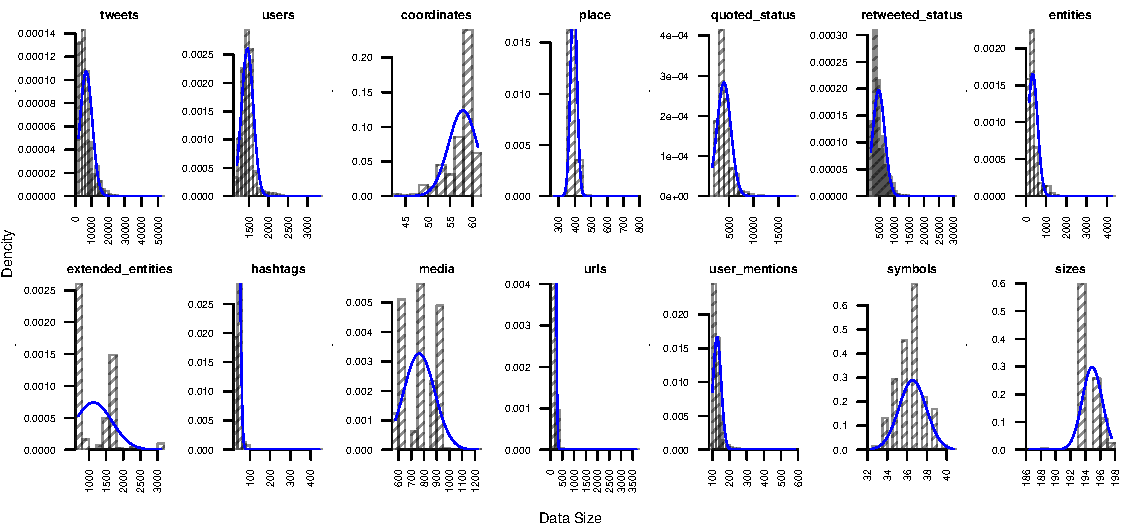
\includegraphics[scale=0.7]{img/Data_Overview.pdf}
	\caption{histograms with Standard Deviation}
	\label{fig:fly}
\end{figure*}
\subsection{References}










\end{document}
